
\subsection{手写面部识别结果}
通过运行proj3.ipynb文件,我们成功实现了基于Dlib和OpenCV的面部识别与换脸功能。
我们选取Elon面部作为源图像,Trump面部作为目标图像,
实验结果展示了从源图像(person1.jpg)到目标图像(person2.jpg)的面部无缝融合。

\subsubsection{面部关键点检测与三角网格可视化}
在换脸过程开始时,需要先检查可视化面部关键点检测和Delaunay三角剖分的结果,结果如图1,2所示。
\begin{figure}
	\centering
	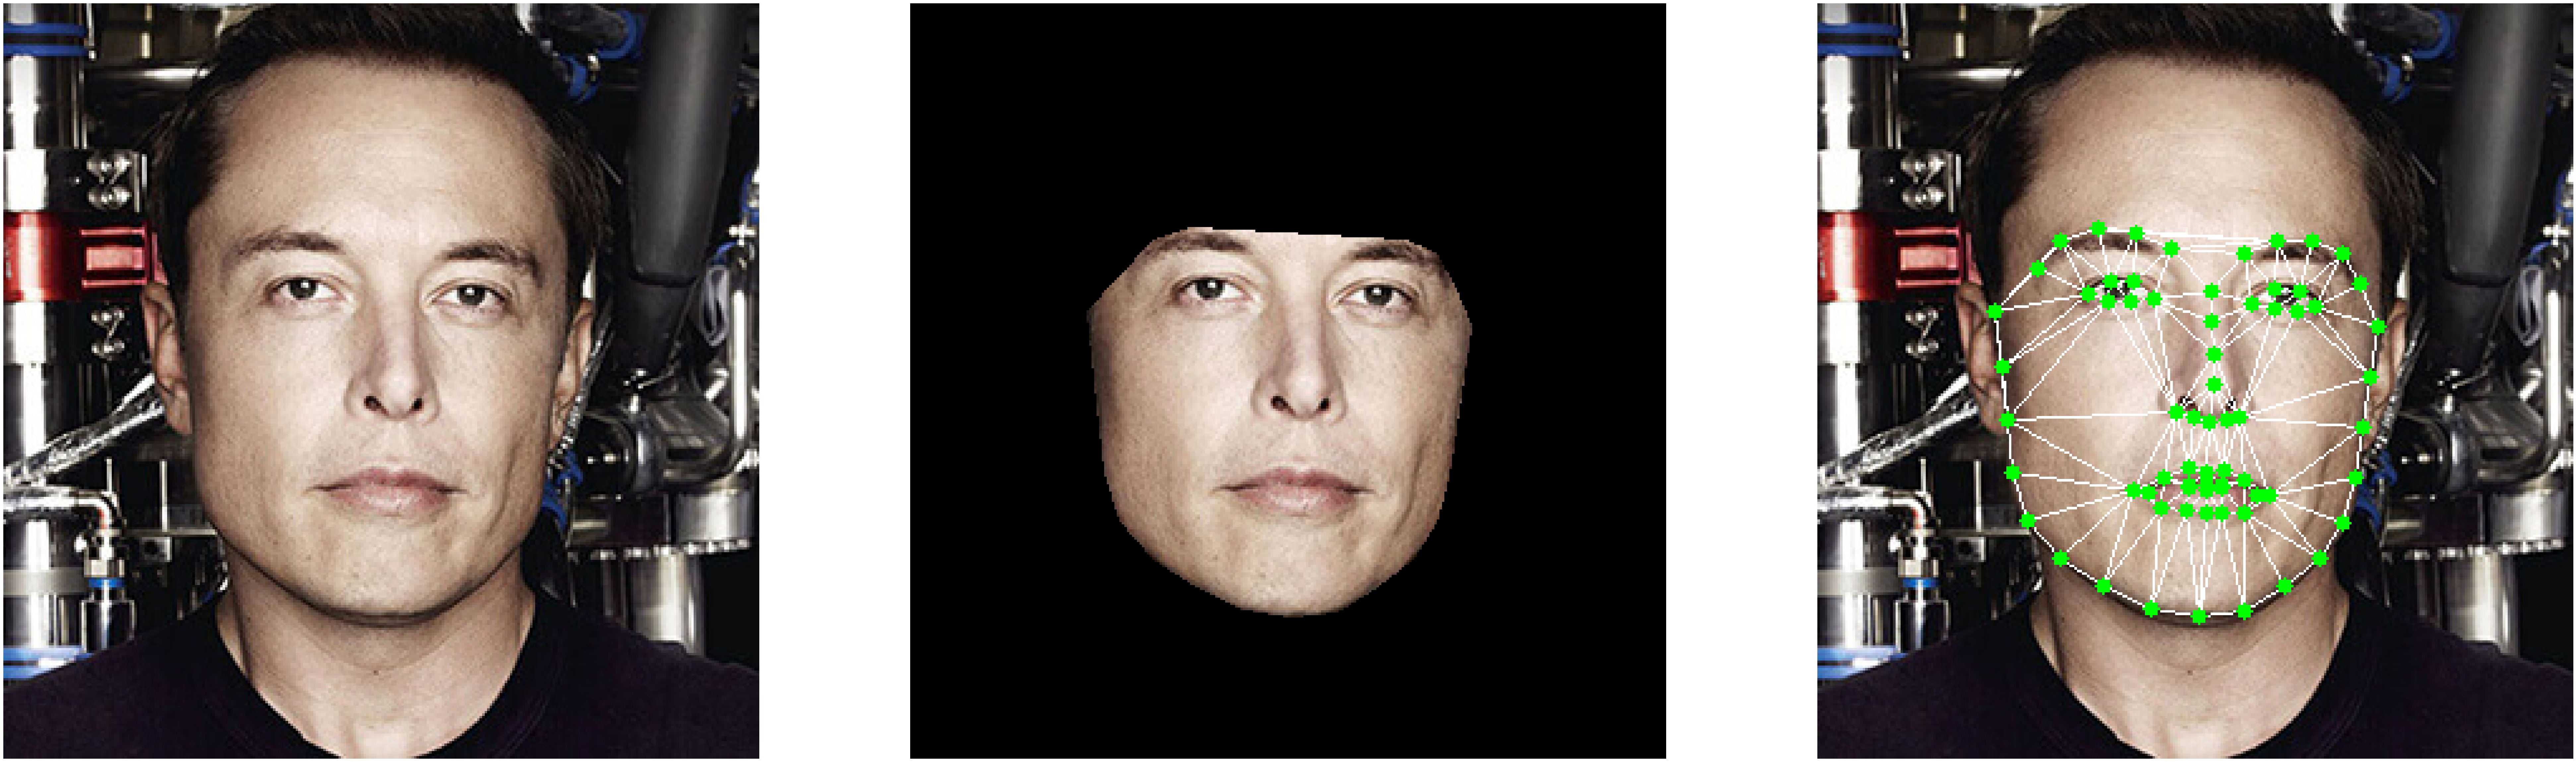
\includegraphics[width=0.7\linewidth]{image/Elon}
	\caption{Elon的面部特征提取}
	\label{图1:}
\end{figure}
\begin{figure}
	\centering
	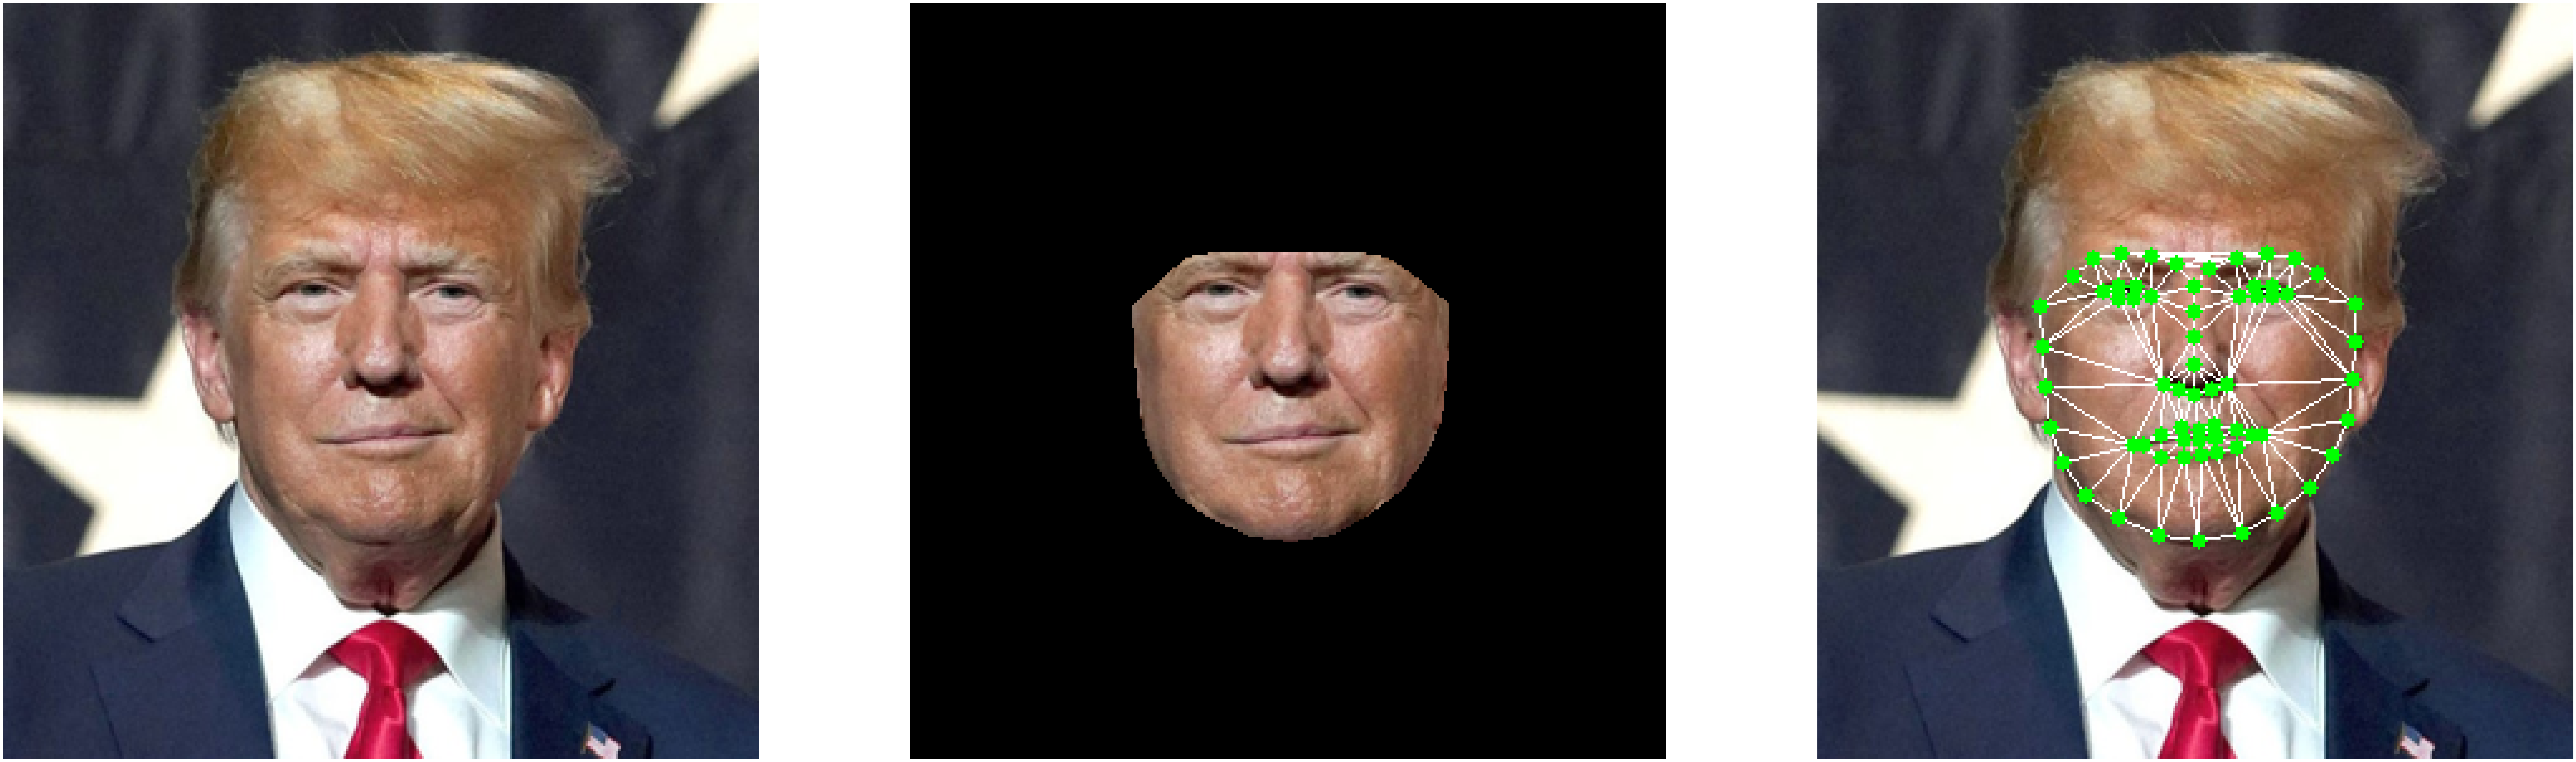
\includegraphics[width=0.7\linewidth]{image/Trump}
	\caption{Trump的面部特征提取}
	\label{图2:}
\end{figure}


\subsubsection{换脸结果}
图3是未经处理的换脸结果。
\begin{figure}
	\centering
	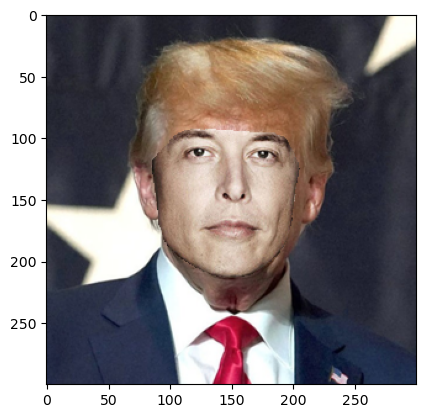
\includegraphics[width=0.7\linewidth]{image/traditional_swap}
	\caption{简单换脸}
	\label{图3:}
\end{figure}

最终的换脸结果通过泊松融合技术实现,确保了源面部与目标图像背景之间的平滑过渡,减少了视觉上的不自然感,如图4所示。
\begin{figure}
	\centering
	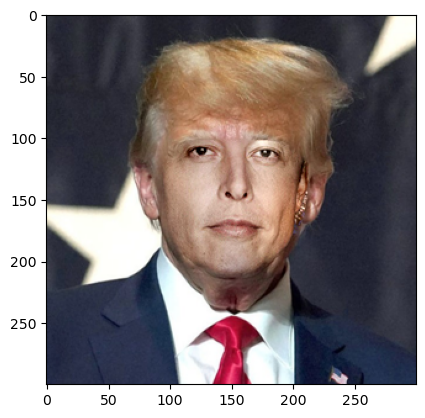
\includegraphics[width=0.7\linewidth]{image/seamlessClone}
	\caption{经过泊松融合之后的结果}
	\label{图4:}
\end{figure}


从结果可以看出,面部特征(如眼睛、鼻子、嘴巴)被成功地从源图像转移到目标图像上,
并且与目标图像的肤色、光照等环境因素进行了较好的融合。

\subsection{大模型换脸}
我们试用了ModelScope平台上的大模型换脸Demo。经过大模型处理后的交换融合结果如图5所示。
\begin{figure}[h!]
    \centering
    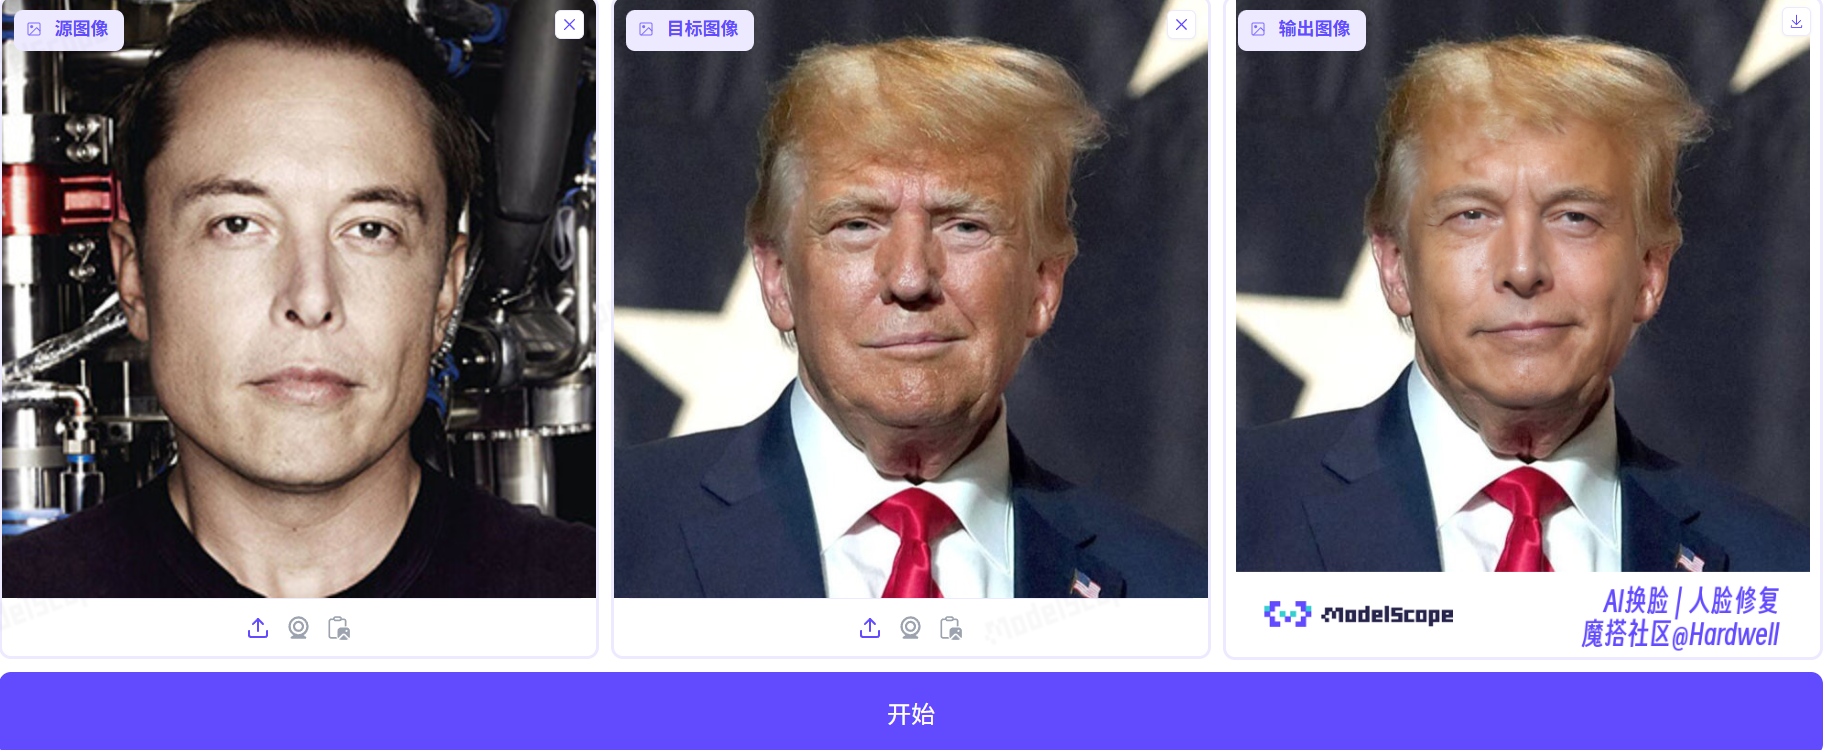
\includegraphics[width=0.8\textwidth]{image/LM_swap.png}
    \caption{大模型换脸结果}
    \label{图5:}
\end{figure}
与手写实现相比,大模型在细节处理和融合自然度方面表现出更高的水平,尤其是在处理复杂光照和面部表情时。
